\documentclass[conference]{IEEEtran}
\IEEEoverridecommandlockouts
% The preceding line is only needed to identify funding in the first footnote. If that is unneeded, please comment it out.
\usepackage{cite}
\usepackage{amsmath,amssymb,amsfonts}
\usepackage{algorithmic}
\usepackage{graphicx}
\usepackage{textcomp}
\usepackage{xcolor}
\usepackage{listings}                           %顯示code用的
\usepackage{fontspec}                           %設定字體
\usepackage[CheckSingle, CJKmath]{xeCJK}
\usepackage{CJKulem}
\usepackage{listings}
\usepackage{color} %red, green, blue, yellow, cyan, magenta, black, white
\usepackage{float}

\definecolor{mygreen}{RGB}{28,172,0} % color values Red, Green, Blue
\definecolor{mylilas}{RGB}{170,55,241}

\setmainfont{Consolas}
%\setmonofont{Ubuntu Mono}
\setmonofont{Consolas}
\setCJKmainfont{Noto Sans CJK TC}
\XeTeXlinebreaklocale "zh"                      %中文自動換行

\lstset{language=Matlab,%
    %basicstyle=\color{red},
    breaklines=true,%
    morekeywords={matlab2tikz},
    keywordstyle=\color{blue},%
    morekeywords=[2]{1}, keywordstyle=[2]{\color{black}},
    identifierstyle=\color{black},%
    stringstyle=\color{mylilas},
    commentstyle=\color{mygreen},%
    showstringspaces=false,%without this there will be a symbol in the places where there is a space
    numbers=left,%
    numberstyle={\tiny \color{black}},% size of the numbers
    numbersep=9pt, % this defines how far the numbers are from the text
    emph=[1]{for,end,break},emphstyle=[1]\color{red}, %some words to emphasise
    %emph=[2]{word1,word2}, emphstyle=[2]{style},    
}

\def\BibTeX{{\rm B\kern-.05em{\sc i\kern-.025em b}\kern-.08em
    T\kern-.1667em\lower.7ex\hbox{E}\kern-.125emX}}

\begin{document}
\title{Digital Image Processing-Assignment 02\\
% {\footnotesize \textsuperscript{*}Note: Sub-titles are not captured in Xplore and should not be used}
% \thanks{Identify applicable funding agency here. If none, delete this.}
}

\author{\IEEEauthorblockN{1\textsuperscript{st} Zih Jie Lin}
\IEEEauthorblockA{\textit{Computer Science Information Engineering.} \\
\textit{Fu Jen Catholoic University}\\
New Taipei City, Taiwan \\
406261597@gapp.fju.edu.tw}
}
% \and
% \IEEEauthorblockN{2\textsuperscript{nd} Given Name Surname}
% \IEEEauthorblockA{\textit{dept. name of organization (of Aff.)} \\
% \textit{name of organization (of Aff.)}\\
% City, Country \\
% email address or ORCID}
% \and
% \IEEEauthorblockN{3\textsuperscript{rd} Given Name Surname}
% \IEEEauthorblockA{\textit{dept. name of organization (of Aff.)} \\
% \textit{name of organization (of Aff.)}\\
% City, Country \\
% email address or ORCID}
% \and
% \IEEEauthorblockN{4\textsuperscript{th} Given Name Surname}
% \IEEEauthorblockA{\textit{dept. name of organization (of Aff.)} \\
% \textit{name of organization (of Aff.)}\\
% City, Country \\
% email address or ORCID}
% \and
% \IEEEauthorblockN{5\textsuperscript{th} Given Name Surname}
% \IEEEauthorblockA{\textit{dept. name of organization (of Aff.)} \\
% \textit{name of organization (of Aff.)}\\
% City, Country \\
% email address or ORCID}
% \and
% \IEEEauthorblockN{6\textsuperscript{th} Given Name Surname}
% \IEEEauthorblockA{\textit{dept. name of organization (of Aff.)} \\
% \textit{name of organization (of Aff.)}\\
% City, Country \\
% email address or ORCID}

\maketitle

% \begin{abstract}
% \end{abstract}

% \begin{IEEEkeywords}
% \end{IEEEkeywords}

\section{實驗說明}
調整 window size, $\sigma$, threshold 參數,觀察是否有改變。

\begin{itemize}
\item window size: $3,5,7$
\item $\sigma$: $0.1,0.3,0.5,0.7,0.9$
\item threshold: $20,30,40,50,60$
\item 圖片: lena, headCT 
\end{itemize}

\section{程式碼}
\lstinputlisting{problem.m}

|\section{Lena}

原圖

\begin{figure}[H]
\centerline{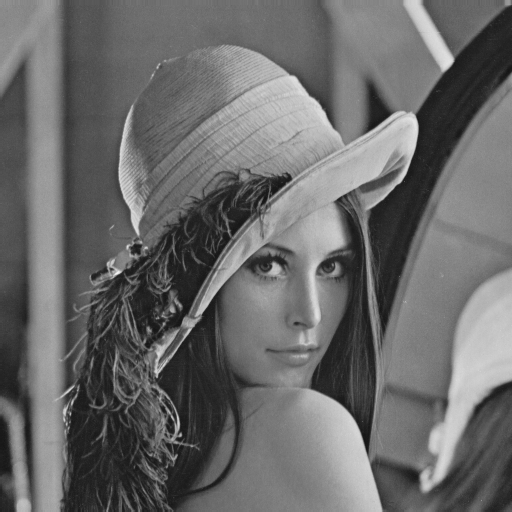
\includegraphics[width=8cm]{lena.png}}
\caption{lena}
\label{lena}
\end{figure}
越大的 threshold 下,白點會明顯地越少。

\begin{figure}[H]
\centerline{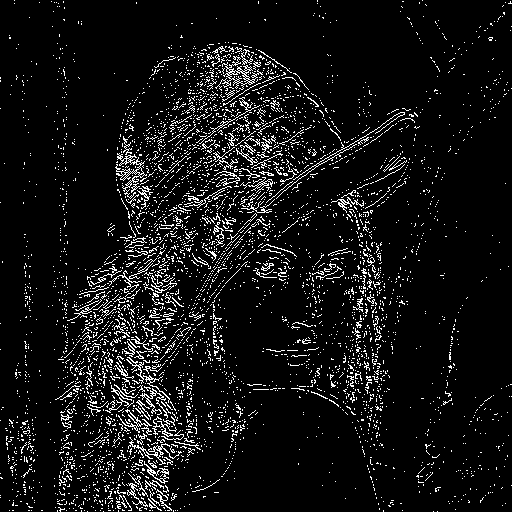
\includegraphics[width=8cm]{lena01.png}}
\caption{window size = $3$, $\sigma=0.1$,  threshold = $20$}
\label{lena01}
\end{figure}

\begin{figure}[H]
\centerline{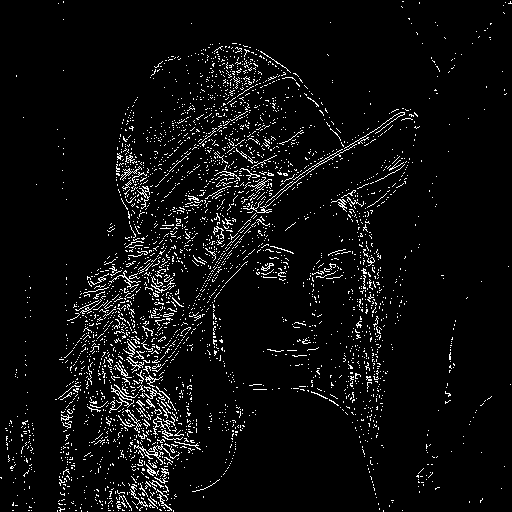
\includegraphics[width=8cm]{lena02.png}}
\caption{window size = $3$, $\sigma=0.1$,  threshold = $30$}
\label{len02}
\end{figure}

\begin{figure}[H]
\centerline{
\includegraphics[width=8cm]{lena03.png}}
\caption{window size = $3$, $\sigma=0.1$,  threshold = $40$}
\label{lena03}
\end{figure}

越大的 $\sigma$ ,邊界的白點會些許的減少。

\begin{figure}[H]
\centerline{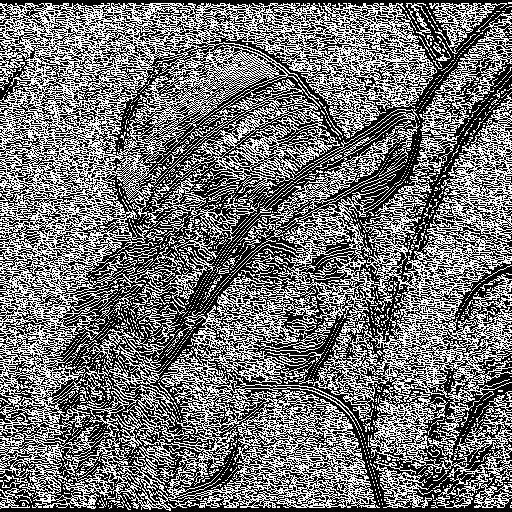
\includegraphics[width=8cm]{lena04.png}}
\caption{window size = $3$, $\sigma=0.3$,  threshold = $40$}
\label{lena04}
\end{figure}

\begin{figure}[H]
\centerline{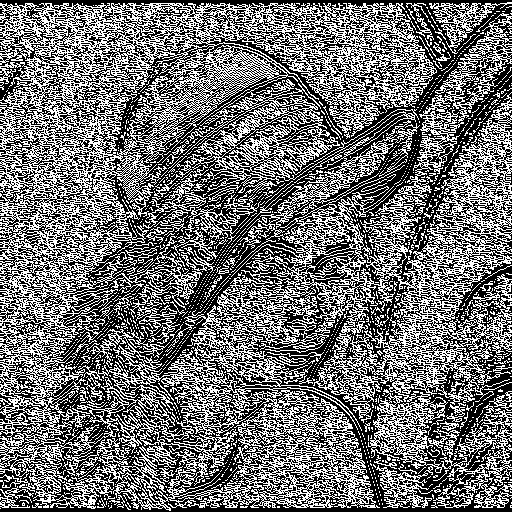
\includegraphics[width=8cm]{lena05.png}}
\caption{window size = $3$, $\sigma=0.5$,  threshold = $40$}
\label{lena05}
\end{figure}

\begin{figure}[H]
\centerline{
\includegraphics[width=8cm]{lena06.png}}
\caption{window size = $3$, $\sigma=0.7$,  threshold = $40$}
\label{lena06}
\end{figure}

\begin{figure}[H]
\centerline{
\includegraphics[width=8cm]{lena07.png}}
\caption{window size = $3$, $\sigma=0.9$,  threshold = $40$}
\label{lena07}
\end{figure}

至於調整不同的 window size,則沒有太大的差異。

\section{headCT}

原圖

\begin{figure}[H]
\centerline{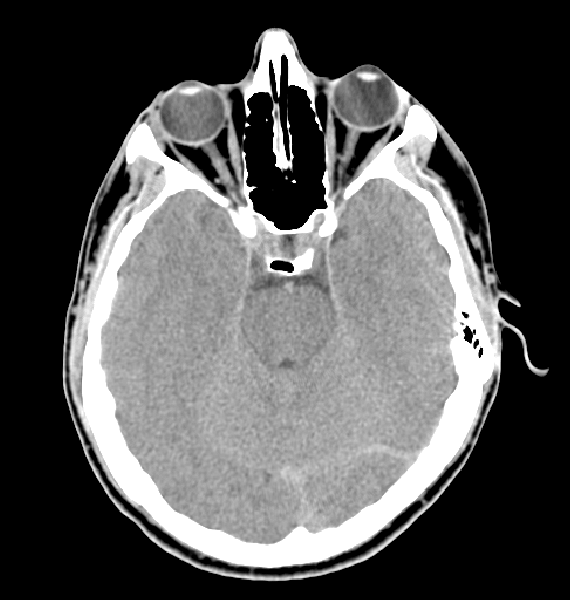
\includegraphics[width=8cm]{headCT.png}}
\caption{headCT}
\label{headCT}
\end{figure}

headCT 圖片情況和 lena 相同。\\

不同的 threshold。

\begin{figure}[H]
\centerline{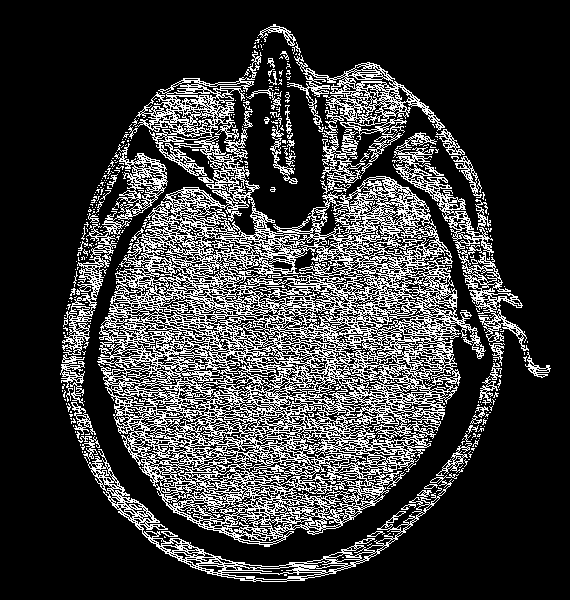
\includegraphics[width=8cm]{headCT01.png}}
\caption{window size = $3$, $\sigma=0.1$,  threshold = $20$}
\label{headCT01}
\end{figure}

\begin{figure}[H]
\centerline{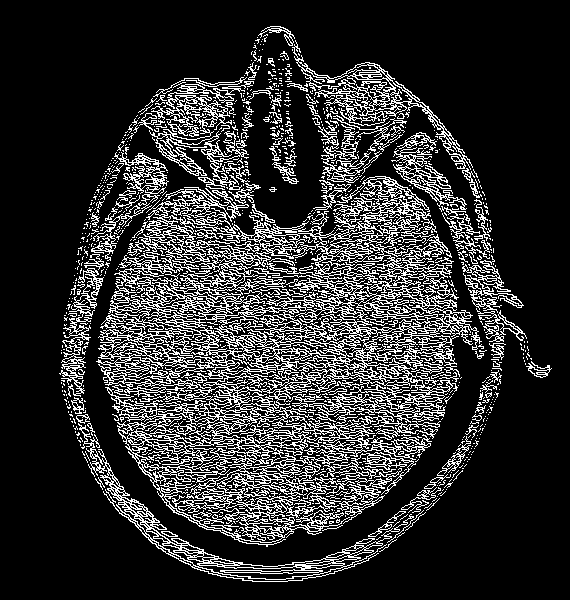
\includegraphics[width=8cm]{headCT02.png}}
\caption{window size = $3$, $\sigma=0.1$,  threshold = $30$}
\label{len02}
\end{figure}

\begin{figure}[H]
\centerline{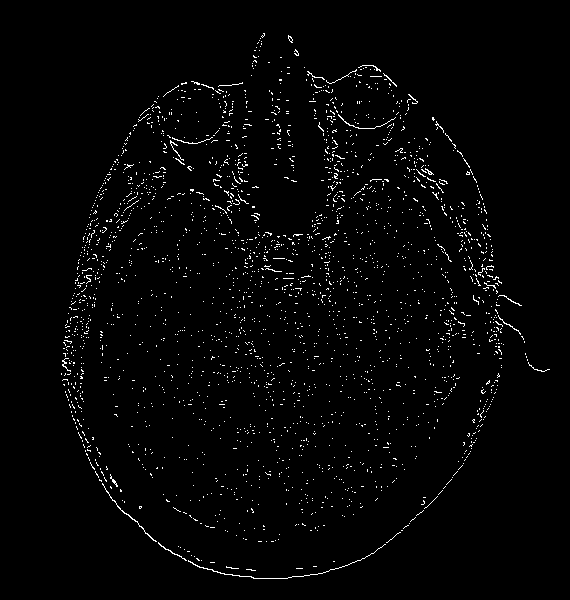
\includegraphics[width=8cm]{headCT03.png}}
\caption{window size = $3$, $\sigma=0.1$,  threshold = $40$}
\label{headCT03}
\end{figure}

不同的 $\sigma$。

\begin{figure}[H]
\centerline{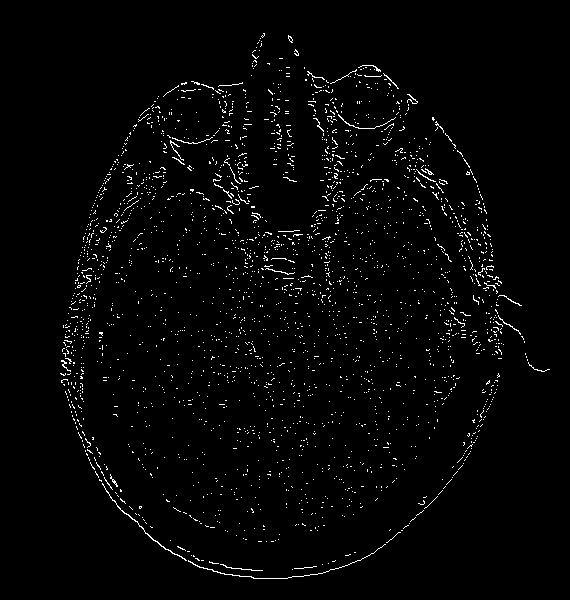
\includegraphics[width=8cm]{headCT04.png}}
\caption{window size = $3$, $\sigma=0.3$,  threshold = $40$}
\label{headCT04}
\end{figure}

\begin{figure}[H]
\centerline{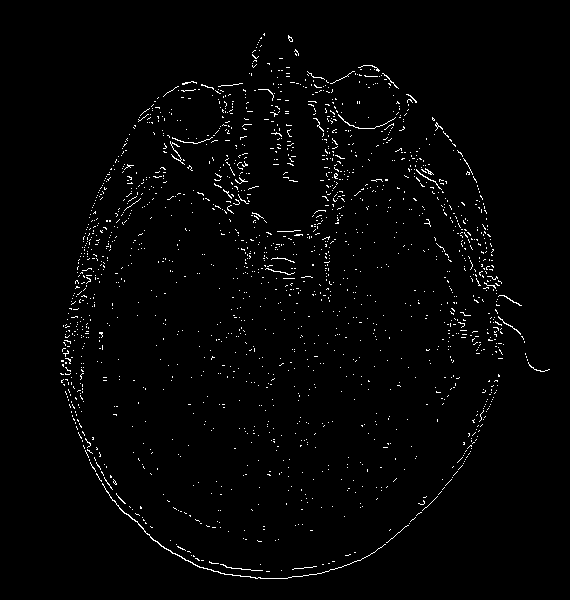
\includegraphics[width=8cm]{headCT05.png}}
\caption{window size = $3$, $\sigma=0.5$,  threshold = $40$}
\label{headCT05}
\end{figure}

\begin{figure}[H]
\centerline{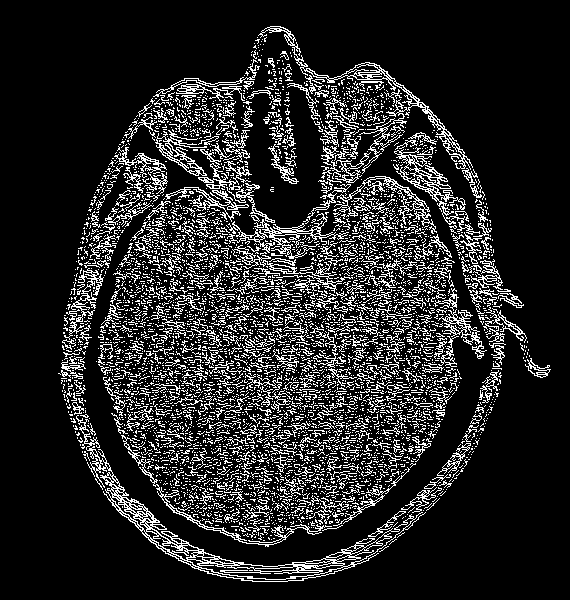
\includegraphics[width=8cm]{headCT06.png}}
\caption{window size = $3$, $\sigma=0.7$,  threshold = $40$}
\label{headCT06}
\end{figure}

\begin{figure}[H]
\centerline{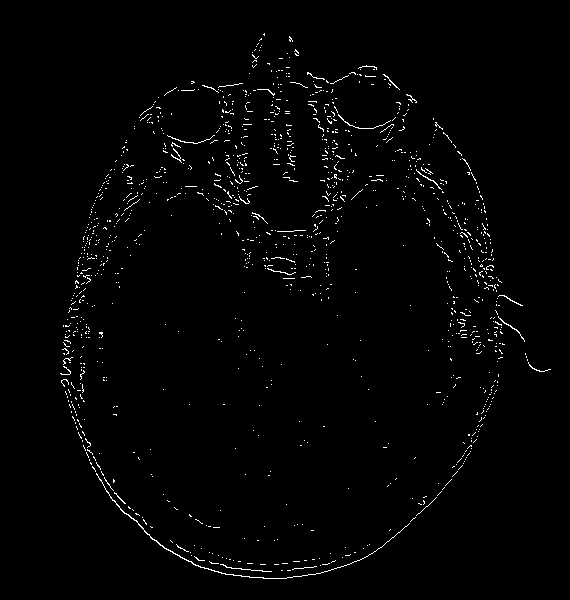
\includegraphics[width=8cm]{headCT07.png}}
\caption{window size = $3$, $\sigma=0.9$,  threshold = $40$}
\label{headCT07}
\end{figure}

% % \begin{thebibliography}{00}
% % \end{thebibliography}

\vspace{12pt}

\end{document}
